
% *** Authors should verify (and, if needed, correct) their LaTeX system  ***
% *** with the testflow diagnostic prior to trusting their LaTeX platform ***
% *** with production work. The IEEE's font choices and paper sizes can   ***
% *** trigger bugs that do not appear when using other class files.       ***                          ***
% The testflow support page is at:
% http://www.michaelshell.org/tex/testflow/
\documentclass[10pt,journal,compsoc]{IEEEtran}
\makeatletter\if@twocolumn\PassOptionsToPackage{switch}{lineno}\else\fi\makeatother


\usepackage{graphicx}
\usepackage[T1]{fontenc}
%
% If IEEEtran.cls has not been installed into the LaTeX system files,
% manually specify the path to it like:
% \documentclass[10pt,journal,compsoc]{../sty/IEEEtran}


% Some very useful LaTeX packages include:
% (uncomment the ones you want to load)


% *** MISC UTILITY PACKAGES ***
%
%\usepackage{ifpdf}
% Heiko Oberdiek's ifpdf.sty is very useful if you need conditional
% compilation based on whether the output is pdf or dvi.
% usage:
% \ifpdf
%   % pdf code
% \else
%   % dvi code
% \fi
% The latest version of ifpdf.sty can be obtained from:
% http://www.ctan.org/pkg/ifpdf
% Also, note that IEEEtran.cls V1.7 and later provides a builtin
% \ifCLASSINFOpdf conditional that works the same way.
% When switching from latex to pdflatex and vice-versa, the compiler may
% have to be run twice to clear warning/error messages.


% *** CITATION PACKAGES ***
%
\ifCLASSOPTIONcompsoc
  % IEEE Computer Society needs nocompress option
  % requires cite.sty v4.0 or later (November 2003)
  \usepackage[nocompress]{cite}
\else
  % normal IEEE
  \usepackage{cite}
\fi
% cite.sty was written by Donald Arseneau
% V1.6 and later of IEEEtran pre-defines the format of the cite.sty package
% \cite{} output to follow that of the IEEE. Loading the cite package will
% result in citation numbers being automatically sorted and properly
% "compressed/ranged". e.g., [1], [9], [2], [7], [5], [6] without using
% cite.sty will become [1], [2], [5]--[7], [9] using cite.sty. cite.sty's
% \cite will automatically add leading space, if needed. Use cite.sty's
% noadjust option (cite.sty V3.8 and later) if you want to turn this off
% such as if a citation ever needs to be enclosed in parenthesis.
% cite.sty is already installed on most LaTeX systems. Be sure and use
% version 5.0 (2009-03-20) and later if using hyperref.sty.
% The latest version can be obtained at:
% http://www.ctan.org/pkg/cite
% The documentation is contained in the cite.sty file itself.
%
% Note that some packages require special options to format as the Computer
% Society requires. In particular, Computer Society  papers do not use
% compressed citation ranges as is done in typical IEEE papers
% (e.g., [1]-[4]). Instead, they list every citation separately in order
% (e.g., [1], [2], [3], [4]). To get the latter we need to load the cite
% package with the nocompress option which is supported by cite.sty v4.0
% and later. Note also the use of a CLASSOPTION conditional provided by
% IEEEtran.cls V1.7 and later.


% *** GRAPHICS RELATED PACKAGES ***
%
\ifCLASSINFOpdf
  %\usepackage[pdftex]{graphicx}
  % declare the path(s) where your graphic files are
  % \graphicspath{{../pdf/}{../jpeg/}}
  % and their extensions so you won't have to specify these with
  % every instance of \includegraphics
  % \DeclareGraphicsExtensions{.pdf,.jpeg,.png}
\else
  % or other class option (dvipsone, dvipdf, if not using dvips). graphicx
  % will default to the driver specified in the system graphics.cfg if no
  % driver is specified.
  % \usepackage[dvips]{graphicx}
  % declare the path(s) where your graphic files are
  % \graphicspath{{../eps/}}
  % and their extensions so you won't have to specify these with
  % every instance of \includegraphics
  % \DeclareGraphicsExtensions{.eps}
\fi
% graphicx was written by David Carlisle and Sebastian Rahtz. It is
% required if you want graphics, photos, etc. graphicx.sty is already
% installed on most LaTeX systems. The latest version and documentation
% can be obtained at: 
% http://www.ctan.org/pkg/graphicx
% Another good source of documentation is "Using Imported Graphics in
% LaTeX2e" by Keith Reckdahl which can be found at:
% http://www.ctan.org/pkg/epslatex
%
% latex, and pdflatex in dvi mode, support graphics in encapsulated
% postscript (.eps) format. pdflatex in pdf mode supports graphics
% in .pdf, .jpeg, .png and .mps (metapost) formats. Users should ensure
% that all non-photo figures use a vector format (.eps, .pdf, .mps) and
% not a bitmapped formats (.jpeg, .png). The IEEE frowns on bitmapped formats
% which can result in "jaggedy"/blurry rendering of lines and letters as
% well as large increases in file sizes.
%
% You can find documentation about the pdfTeX application at:
% http://www.tug.org/applications/pdftex


% *** MATH PACKAGES ***
%
\usepackage{amsmath}
\usepackage[cmintegrals]{newtxmath}
% A popular package from the American Mathematical Society that provides
% many useful and powerful commands for dealing with mathematics.
%
% Note that the amsmath package sets \interdisplaylinepenalty to 10000
% thus preventing page breaks from occurring within multiline equations. Use:
\interdisplaylinepenalty=2500
% after loading amsmath to restore such page breaks as IEEEtran.cls normally
% does. amsmath.sty is already installed on most LaTeX systems. The latest
% version and documentation can be obtained at:
% http://www.ctan.org/pkg/amsmath


% *** SPECIALIZED LIST PACKAGES ***
%
%\usepackage{algorithmic}
% algorithmic.sty was written by Peter Williams and Rogerio Brito.
% This package provides an algorithmic environment fo describing algorithms.
% You can use the algorithmic environment in-text or within a figure
% environment to provide for a floating algorithm. Do NOT use the algorithm
% floating environment provided by algorithm.sty (by the same authors) or
% algorithm2e.sty (by Christophe Fiorio) as the IEEE does not use dedicated
% algorithm float types and packages that provide these will not provide
% correct IEEE style captions. The latest version and documentation of
% algorithmic.sty can be obtained at:
% http://www.ctan.org/pkg/algorithms
% Also of interest may be the (relatively newer and more customizable)
% algorithmicx.sty package by Szasz Janos:
% http://www.ctan.org/pkg/algorithmicx


% *** ALIGNMENT PACKAGES ***
%
%\usepackage{array}
% Frank Mittelbach's and David Carlisle's array.sty patches and improves
% the standard LaTeX2e array and tabular environments to provide better
% appearance and additional user controls. As the default LaTeX2e table
% generation code is lacking to the point of almost being broken with
% respect to the quality of the end results, all users are strongly
% advised to use an enhanced (at the very least that provided by array.sty)
% set of table tools. array.sty is already installed on most systems. The
% latest version and documentation can be obtained at:
% http://www.ctan.org/pkg/array


% IEEEtran contains the IEEEeqnarray family of commands that can be used to
% generate multiline equations as well as matrices, tables, etc., of high
% quality.


% *** SUBFIGURE PACKAGES ***
%\ifCLASSOPTIONcompsoc
%  \usepackage[caption=false,font=footnotesize,labelfont=sf,textfont=sf]{subfig}
%\else
%  \usepackage[caption=false,font=footnotesize]{subfig}
%\fi
% subfig.sty, written by Steven Douglas Cochran, is the modern replacement
% for subfigure.sty, the latter of which is no longer maintained and is
% incompatible with some LaTeX packages including fixltx2e. However,
% subfig.sty requires and automatically loads Axel Sommerfeldt's caption.sty
% which will override IEEEtran.cls' handling of captions and this will result
% in non-IEEE style figure/table captions. To prevent this problem, be sure
% and invoke subfig.sty's "caption=false" package option (available since
% subfig.sty version 1.3, 2005/06/28) as this is will preserve IEEEtran.cls
% handling of captions.
% Note that the Computer Society format requires a sans serif font rather
% than the serif font used in traditional IEEE formatting and thus the need
% to invoke different subfig.sty package options depending on whether
% compsoc mode has been enabled.
%
% The latest version and documentation of subfig.sty can be obtained at:
% http://www.ctan.org/pkg/subfig


% *** FLOAT PACKAGES ***
%
%\usepackage{fixltx2e}
% fixltx2e, the successor to the earlier fix2col.sty, was written by
% Frank Mittelbach and David Carlisle. This package corrects a few problems
% in the LaTeX2e kernel, the most notable of which is that in current
% LaTeX2e releases, the ordering of single and double column floats is not
% guaranteed to be preserved. Thus, an unpatched LaTeX2e can allow a
% single column figure to be placed prior to an earlier double column
% figure.
% Be aware that LaTeX2e kernels dated 2015 and later have fixltx2e.sty's
% corrections already built into the system in which case a warning will
% be issued if an attempt is made to load fixltx2e.sty as it is no longer
% needed.
% The latest version and documentation can be found at:
% http://www.ctan.org/pkg/fixltx2e


%\usepackage{stfloats}
% stfloats.sty was written by Sigitas Tolusis. This package gives LaTeX2e
% the ability to do double column floats at the bottom of the page as well
% as the top. (e.g., "\begin{figure*}[!b]" is not normally possible in
% LaTeX2e). It also provides a command:
%\fnbelowfloat
% to enable the placement of footnotes below bottom floats (the standard
% LaTeX2e kernel puts them above bottom floats). This is an invasive package
% which rewrites many portions of the LaTeX2e float routines. It may not work
% with other packages that modify the LaTeX2e float routines. The latest
% version and documentation can be obtained at:
% http://www.ctan.org/pkg/stfloats
% Do not use the stfloats baselinefloat ability as the IEEE does not allow
% \baselineskip to stretch. Authors submitting work to the IEEE should note
% that the IEEE rarely uses double column equations and that authors should try
% to avoid such use. Do not be tempted to use the cuted.sty or midfloat.sty
% packages (also by Sigitas Tolusis) as the IEEE does not format its papers in
% such ways.
% Do not attempt to use stfloats with fixltx2e as they are incompatible.
% Instead, use Morten Hogholm'a dblfloatfix which combines the features
% of both fixltx2e and stfloats:
%
% \usepackage{dblfloatfix}
% The latest version can be found at:
% http://www.ctan.org/pkg/dblfloatfix


%\ifCLASSOPTIONcaptionsoff
%  \usepackage[nomarkers]{endfloat}
% \let\MYoriglatexcaption\caption
% \renewcommand{\caption}[2][\relax]{\MYoriglatexcaption[#2]{#2}}
%\fi
% endfloat.sty was written by James Darrell McCauley, Jeff Goldberg and 
% Axel Sommerfeldt. This package may be useful when used in conjunction with 
% IEEEtran.cls'  captionsoff option. Some IEEE journals/societies require that
% submissions have lists of figures/tables at the end of the paper and that
% figures/tables without any captions are placed on a page by themselves at
% the end of the document. If needed, the draftcls IEEEtran class option or
% \CLASSINPUTbaselinestretch interface can be used to increase the line
% spacing as well. Be sure and use the nomarkers option of endfloat to
% prevent endfloat from "marking" where the figures would have been placed
% in the text. The two hack lines of code above are a slight modification of
% that suggested by in the endfloat docs (section 8.4.1) to ensure that
% the full captions always appear in the list of figures/tables - even if
% the user used the short optional argument of \caption[]{}.
% IEEE papers do not typically make use of \caption[]'s optional argument,
% so this should not be an issue. A similar trick can be used to disable
% captions of packages such as subfig.sty that lack options to turn off
% the subcaptions:
% For subfig.sty:
% \let\MYorigsubfloat\subfloat
% \renewcommand{\subfloat}[2][\relax]{\MYorigsubfloat[]{#2}}
% However, the above trick will not work if both optional arguments of
% the \subfloat command are used. Furthermore, there needs to be a
% description of each subfigure *somewhere* and endfloat does not add
% subfigure captions to its list of figures. Thus, the best approach is to
% avoid the use of subfigure captions (many IEEE journals avoid them anyway)
% and instead reference/explain all the subfigures within the main caption.
% The latest version of endfloat.sty and its documentation can obtained at:
% http://www.ctan.org/pkg/endfloat
%
% The IEEEtran \ifCLASSOPTIONcaptionsoff conditional can also be used
% later in the document, say, to conditionally put the References on a 
% page by themselves.


% *** PDF, URL AND HYPERLINK PACKAGES ***
%
\usepackage{url}
% url.sty was written by Donald Arseneau. It provides better support for
% handling and breaking URLs. url.sty is already installed on most LaTeX
% systems. The latest version and documentation can be obtained at:
% http://www.ctan.org/pkg/url
% Basically, \url{my_url_here}.


% *** Do not adjust lengths that control margins, column widths, etc. ***
% *** Do not use packages that alter fonts (such as pslatex).         ***
% There should be no need to do such things with IEEEtran.cls V1.6 and later.
% (Unless specifically asked to do so by the journal or conference you plan
% to submit to, of course. )


% correct bad hyphenation here
\hyphenation{op-tical net-works semi-conduc-tor}

%%%%%%%%%%%%%%%%%%%%%%%%%%%%%%%%%%%%%%%%%%%%%%%%%%%%%%%%%%%%%%%%%%%%%%%%%%
% Following additional macros are required to function some 
% functions which are not available in the class used.
%%%%%%%%%%%%%%%%%%%%%%%%%%%%%%%%%%%%%%%%%%%%%%%%%%%%%%%%%%%%%%%%%%%%%%%%%%
\usepackage{url,multirow,morefloats,floatflt,cancel,tfrupee}
\makeatletter


\AtBeginDocument{\@ifpackageloaded{textcomp}{}{\usepackage{textcomp}}}
\makeatother
\usepackage{colortbl}
\usepackage{xcolor}
\usepackage{pifont}
\usepackage[nointegrals]{wasysym}
\urlstyle{rm}
\makeatletter

%%%For Table column width calculation.
\def\mcWidth#1{\csname TY@F#1\endcsname+\tabcolsep}

%%Hacking center and right align for table
\def\cAlignHack{\rightskip\@flushglue\leftskip\@flushglue\parindent\z@\parfillskip\z@skip}
\def\rAlignHack{\rightskip\z@skip\leftskip\@flushglue \parindent\z@\parfillskip\z@skip}

%Etal definition in references
\@ifundefined{etal}{\def\etal{\textit{et~al}}}{}


%\if@twocolumn\usepackage{dblfloatfix}\fi
\usepackage{ifxetex}
\ifxetex\else\if@twocolumn\@ifpackageloaded{stfloats}{}{\usepackage{dblfloatfix}}\fi\fi

\AtBeginDocument{
\expandafter\ifx\csname eqalign\endcsname\relax
\def\eqalign#1{\null\vcenter{\def\\{\cr}\openup\jot\m@th
  \ialign{\strut$\displaystyle{##}$\hfil&$\displaystyle{{}##}$\hfil
      \crcr#1\crcr}}\,}
\fi
}

%For fixing hardfail when unicode letters appear inside table with endfloat
\AtBeginDocument{%
  \@ifpackageloaded{endfloat}%
   {\renewcommand\efloat@iwrite[1]{\immediate\expandafter\protected@write\csname efloat@post#1\endcsname{}}}{\newif\ifefloat@tables}%
}%

\def\BreakURLText#1{\@tfor\brk@tempa:=#1\do{\brk@tempa\hskip0pt}}
\let\lt=<
\let\gt=>
\def\processVert{\ifmmode|\else\textbar\fi}
\let\processvert\processVert

\@ifundefined{subparagraph}{
\def\subparagraph{\@startsection{paragraph}{5}{2\parindent}{0ex plus 0.1ex minus 0.1ex}%
{0ex}{\normalfont\small\itshape}}%
}{}

% These are now gobbled, so won't appear in the PDF.
\newcommand\role[1]{\unskip}
\newcommand\aucollab[1]{\unskip}
  
\@ifundefined{tsGraphicsScaleX}{\gdef\tsGraphicsScaleX{1}}{}
\@ifundefined{tsGraphicsScaleY}{\gdef\tsGraphicsScaleY{.9}}{}
% To automatically resize figures to fit inside the text area
\def\checkGraphicsWidth{\ifdim\Gin@nat@width>\linewidth
	\tsGraphicsScaleX\linewidth\else\Gin@nat@width\fi}

\def\checkGraphicsHeight{\ifdim\Gin@nat@height>.9\textheight
	\tsGraphicsScaleY\textheight\else\Gin@nat@height\fi}

\def\fixFloatSize#1{}%\@ifundefined{processdelayedfloats}{\setbox0=\hbox{\includegraphics{#1}}\ifnum\wd0<\columnwidth\relax\renewenvironment{figure*}{\begin{figure}}{\end{figure}}\fi}{}}
\let\ts@includegraphics\includegraphics

\def\inlinegraphic[#1]#2{{\edef\@tempa{#1}\edef\baseline@shift{\ifx\@tempa\@empty0\else#1\fi}\edef\tempZ{\the\numexpr(\numexpr(\baseline@shift*\f@size/100))}\protect\raisebox{\tempZ pt}{\ts@includegraphics{#2}}}}

%\renewcommand{\includegraphics}[1]{\ts@includegraphics[width=\checkGraphicsWidth]{#1}}
\AtBeginDocument{\def\includegraphics{\@ifnextchar[{\ts@includegraphics}{\ts@includegraphics[width=\checkGraphicsWidth,height=\checkGraphicsHeight,keepaspectratio]}}}

\DeclareMathAlphabet{\mathpzc}{OT1}{pzc}{m}{it}

\def\URL#1#2{\@ifundefined{href}{#2}{\href{#1}{#2}}}

%%For url break
\def\UrlOrds{\do\*\do\-\do\~\do\'\do\"\do\-}%
\g@addto@macro{\UrlBreaks}{\UrlOrds}



\edef\fntEncoding{\f@encoding}
\def\EUoneEnc{EU1}
\makeatother
\def\floatpagefraction{0.8} 
\def\dblfloatpagefraction{0.8}
\def\style#1#2{#2}
\def\xxxguillemotleft{\fontencoding{T1}\selectfont\guillemotleft}
\def\xxxguillemotright{\fontencoding{T1}\selectfont\guillemotright}

\newif\ifmultipleabstract\multipleabstractfalse%
\newenvironment{typesetAbstractGroup}{}{}%

%%%%%%%%%%%%%%%%%%%%%%%%%%%%%%%%%%%%%%%%%%%%%%%%%%%%%%%%%%%%%%%%%%%%%%%%%%

\makeatletter
\AtBeginDocument{\@ifpackageloaded{longtable}{%
\def\LT@makecaption#1#2#3{%
  \LT@mcol\LT@cols c{\hbox to\z@{\hss\parbox[t]\LTcapwidth{%
    \sbox\@tempboxa{#1{#2: } #3}%
    \ifdim\wd\@tempboxa>\hsize
      #1{#2: }\textsc{#3}%
    \else
      \hbox to\hsize{\hfil\box\@tempboxa\hfil}%
    \fi
    \endgraf\vskip\baselineskip}%
  \hss}}}
}{}}
\makeatother



%% *** Changes ***
\usepackage{tikz}
\usepackage{xcolor}
\newcommand*\circled[2][]{\tikz[baseline=(char.base)]{
    \node[shape=circle,draw,inner sep=2pt,{#1},every number/.try] (char) {\color{white}#2};}}
\tikzstyle{every number}=[draw=black] % I like to use tikzstyle ;)

\usepackage{stackengine}
\newcommand\xrowht[2][0]{\addstackgap[.5\dimexpr#2\relax]{\vphantom{#1}}}
%% *** Changes ***


\begin{document}


%
% paper title
% Titles are generally capitalized except for words such as a, an, and, as,
% at, but, by, for, in, nor, of, on, or, the, to and up, which are usually
% not capitalized unless they are the first or last word of the title.
% Linebreaks \\ can be used within to get better formatting as desired.
% Do not put math or special symbols in the title.
\title{Tabla: A framework for Extracting Tables From Images}
% author names and IEEE memberships
\author{Ayush~Jain\IEEEcompsocitemizethanks{\IEEEcompsocthanksitem {Ayush Jain: 16116013}}, Shubanshu~Agarwal\IEEEcompsocitemizethanks{\IEEEcompsocthanksitem Shubhanshu Agarwal: 161160XX}, Suyash~Mahar\IEEEcompsocitemizethanks{\IEEEcompsocthanksitem Suyash Mahar: 16116069}}

\IEEEtitleabstractindextext{
\begin{abstract}
Extracting tables from images is a very important task but has limited open source support, currently available frameworks are limited in either performance or usability. The aim of this work is to create a new framework that improves usability while producing high-quality results. We use basic image processing techniques like erosion/dilation, binarization, adaptive thresholding and inversion along with optimizations for broken and misaligned lines to show how even simple methods can result in high-quality results. We find that our tool while being extremely user-friendly in the sense that it doesn't require any tuning from the user, produces high quality results and also supports extracting merged cells in a table. These requirements make Tabla a powerful and versatile tool. Thus we hope that Tabla would help ease the effort required to extract tables from images by being user-friendly as it doesn't require and input other than the image and by using simple image processing to create accurate results.
\end{abstract}
    
\begin{IEEEkeywords}
Table Extraction, OCR, Image Processing 
\end{IEEEkeywords}
}

% make the title area
\maketitle 
      
% To allow for easy dual compilation without having to reenter the
% abstract/keywords data, the \IEEEtitleabstractindextext text will
% not be used in maketitle, but will appear (i.e., to be "transported")
% here as \IEEEdisplaynontitleabstractindextext when the compsoc 
% or transmag modes are not selected <OR> if conference mode is selected 
% - because all conference papers position the abstract like regular
% papers do.
\IEEEdisplaynontitleabstractindextext
% \IEEEdisplaynontitleabstractindextext has no effect when using
% compsoc or transmag under a non-conference mode.

% For peer review papers, you can put extra information on the cover
% page as needed:
% \ifCLASSOPTIONpeerreview
% \begin{center} \bfseries EDICS Category: 3-BBND \end{center}
% \fi
%
% For peerreview papers, this IEEEtran command inserts a page break and
% creates the second title. It will be ignored for other modes.
\IEEEpeerreviewmaketitle



\newcommand{\inline}[1]{\texttt{#1}}
    
\section{Introduction}
The need for Tabla arose from the fact that current open source table extractors are severely limited in terms of their performance, the limitations of two of the most popular implementations are listed below:

\begin{itemize}
\item \textbf{pdftabextract}\cite{Konrad2017GitHub, Konrad2017Blog} This framework was developed as a tool to accelerate extraction of information for analysing and archiving, however it suffers from the following major limitations:
\begin{itemize}
    \item The framework's performance is limited when a number of fine lines are present in the image, it also classifies text as table border when letter spacing is less than the usual amount.
    \item Another limitation is the manual input required by the user for every image to tune the hyper-parameters of the algorithm, this severely limits the usability and hampers productivity.
\end{itemize}

\item \textbf{Tabula}\cite{tabula2018} This is a full-fledged package for extracting information (i.e. we cannot get intermediate results), however this package suffers from some serious limitation:
\begin{itemize}
    \item This framework works only if the text is already embedded in the PDF file and there is no open-source tool available to detect text and embed it directly into the PDF file. This has also been an open GitHub issue on its repository. \cite{tabula2018issue}.
\end{itemize}
\end{itemize}

Thus, we present `Tabla', a framework that overcomes all these limitation by the use of simple image processing algorithms and techniques to extract table from an image. Tabla does so without any manual input from the user, easing usability and is highly accurate for images where other frameworks/algorithms fail.

The rest of the paper is: Section 2 talks about how different existing technologies are used, this is followed by detailed explanation of the working of Tabla in Section 3 and finally the results are presented in Section 4.

    
\section{Technology}

\begin{table}[!h]
\renewcommand{\arraystretch}{1.3}
\caption{Overview of the technologies used}
\label{table_example}
\centering
\begin{tabular}{|c||c|}
\hline
\textbf{Language} & C++ 2011 Standard\\
\hline
\textbf{Build Tool} & CMake (Minimum version 3.10)\\
\hline
\end{tabular}
\end{table}

\subsection{OpenCV\cite{opencv_library}}
OpenCV being a very powerful tool is extensively used across our project for a wide variety of tasks, some of them are:
\begin{itemize}
    \item Binary inversion with adaptive Gaussian noise removal filter.
    \item Contour mapping for identifying the table borders.
    \item \textbf{Morphological operations:} Erosion and Dilation \cite{gonzalez2002richard} to anything except corresponding to a particular direction, either horizontal or vertical.
    \item Custom operations over OpenCV matrix of the secluded horizontal lines image and the secluded vertical lines image to extract line coordinates.
\end{itemize}
\subsection{Tesseract-OCR\cite{googleTesseract}}
We also make extensive use of the \inline{tesseract-ocr} library for the following purposes:
\begin{itemize}
    \item Detecting of blocks of words in the image.
    \item Detecting bounding boxes of each block of words.
    \item Language specific (by default, English) LSTM prediction in OCR.
\end{itemize}


\section{Working}
\begin{figure*}[!t]
\centering
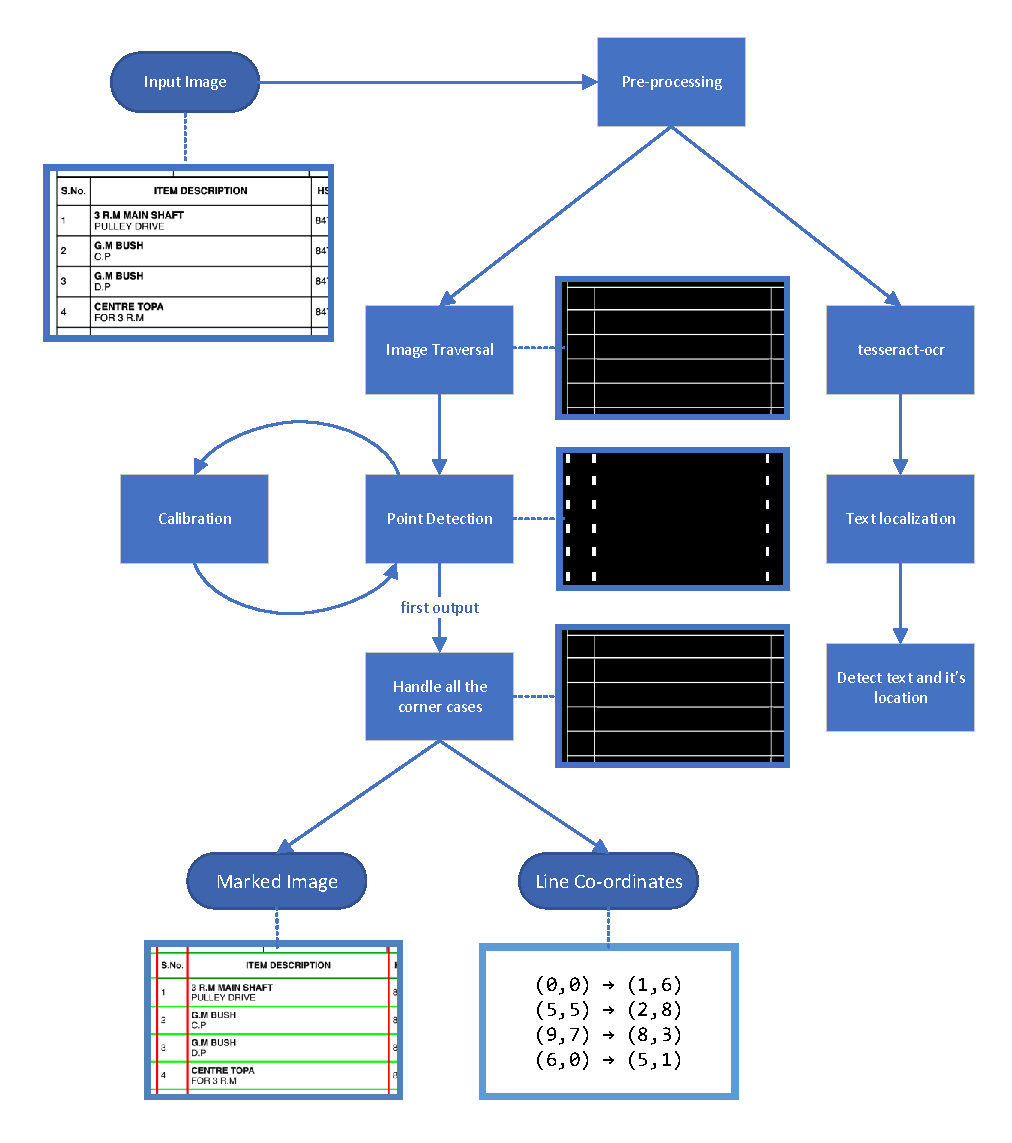
\includegraphics[width=0.8\textwidth]{figures/overview.pdf}
\caption{Overview of the tabla algorithm with an example demonstrating various operations performed on the image.}
\label{fig:overview}
\end{figure*}

\begin{figure*}[!t]
\centering
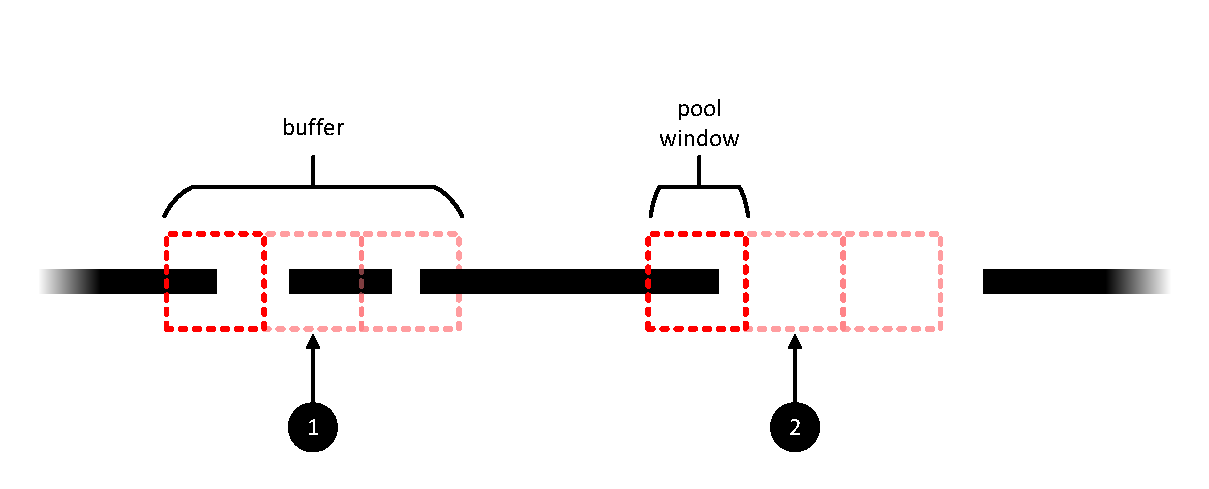
\includegraphics[width=0.7\textwidth]{figures/buffer.pdf}
\caption{Application of pool buffer. Checking the subsequent pool windows indicates whether it's an endpoint or a minor glitch. In \circled[fill=black]{1}: the buffer detects non-zero values in next pool windows, thus, indicating a glitch. And in \circled[fill=black]{2}: the buffer detects no values in the next pool windows, indicating that the current one is an endpoint.}
\label{fig:buffer}
\end{figure*}

\begin{figure}[!t]
\centering
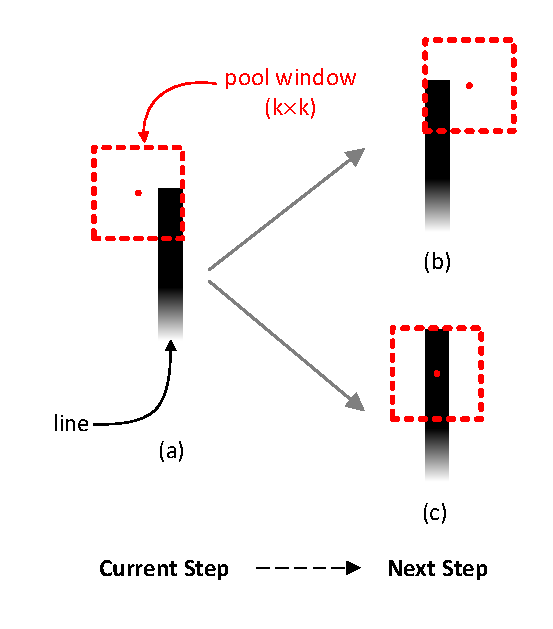
\includegraphics[width=2.5in]{figures/calibration.pdf}
\caption{Tabla calibrates the pool window to prevent windows with lower than threshold line content to be skipped. (a) Current state of the pool window. Notice how the line's end lies at the extreme corner. (b) \textbf{Without calibration:} Pool window might skip the detected region. (c) \textbf{With calibration:} Pool window calibrates to match its centre.}
\label{fig:calibration}
\end{figure}

\begin{figure}[!t]
\centering
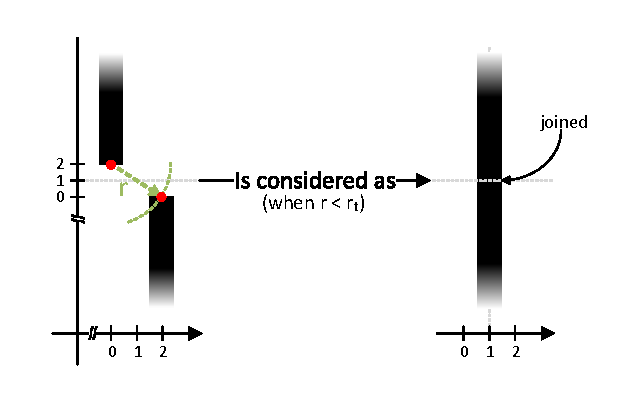
\includegraphics[width=0.45\textwidth]{figures/cleanLines.pdf}
\caption{Tabla merges lines that have distance between their endpoints and centre points on one of the axes, less than a certain thresholds.}
\label{fig:cleanLines}
\end{figure}

\subsection{Pre-processing}
The most important tool used to build this project is OpenCV, an open-source library written in C/C++ with highly optimized algorithms. It has support for almost all the traditional image processing algorithms, as well as, interfaces and modules to use deep learning techniques. For text character recognition, Google's \inline{tesseract-ocr} is being used with customized settings so as to not only detect the word blocks but the pixel coordinates of their bounding boxes too.

\subsubsection{Reading an Image}
Recommended image type is \textit{Portable Network Graphics (PNG)} for proper recognition of pixel data in case of character recognition. Since a very high-resolution image will increase the execution time, it is expected the image resolution is not greater than ~0.4MP.

\subsubsection{Grayscaling}
To reduce the computational complexity of processing an image, a three-channel RGB image is converted to greyscale using OpenCV, which uses the following relation
\begin{equation}
    Y = 0.299R + 0.587G + 0.114B
\end{equation}

\subsubsection{Preparing the image}
Real world data is noisy, and a scanned image can have varying intensity in the background itself due to noise in the scanner or cleanliness of the paper that is to be scanned. Since an image of a text-only table does not require intensity variations for distinguishing the data from its background. Thus, the image is binarized with thresholds defined using \textit{adaptive thresholding}, that calculates different thresholds for small chunks of the image, thereby, increasing the accuracy of image binarization for images having varying illumination.

% After pre-processing the image, the inverted and binarized image is then sent to two pipelines, one for extracting and locating the edges, and the other to recognize the text as blocks of words along with their location in the image.

\subsection{Morphological operations}
An important step to recognize the table structure in the image is to segregate all the horizontal and vertical structures. Morphological operations like \textit{erosion} and \textit{dilation} when applied with proper kernels can extract straight lines along both the axes.

In case of a curve deviating from the structuring element, an \textit{erosion} operation will remove all the pixel data from that small chunk on which the kernel is applied. Otherwise, for a linear curve along the structuring element that is completely covering the kernel, all the pixel data is set to the maximum value present. The subsequent dilation operation then smooths out the data along the structure by setting the values to maximum if the line is present.

\subsection{Edge Recognition and Localization}
After segregating the horizontal lines and vertical lines, it is required to localize the endpoints of all the lines, so that, when compared to the detected text's location, the corresponding table cell location can be deduced.

\subsubsection{Image traversal}
The image is traversed by looping a \textit{pool window}, $k{\times}k$ kernel, like a look-up lens, on which all the subsequent operations will be executed. This means some linear function over all the grayscale values of the pixels present in the pool will decide whether the centre point represents an endpoint and/or what must be the next step. The traversal of the pool window reduces the complexity as compared to the pixel by pixel traversal.

\subsubsection{Detection of end points}
A start point, in this case, can be defined as the location of the centre of the pool window for the first time when the white region\footnote{For aesthetic purposes, illustrations present in the region have black lines over white background. In the project, the image is binary inverted.} appears. The appearance of the white region means that it can either be a part of some line or some noise. For acknowledging the endpoint, a threshold is set for the number of white pixels in the white region. Moreover, a buffer of some $n$ number of pool windows is checked if they have crossed the threshold or not. This helps in handling minor glitches or small discontinuities present on the line. Figure \ref{fig:buffer} explains how introducing a buffer of $n=3$ pool windows to check for the required region can help in ignoring noise or glitches. Similarly, for locating the end point, the first time when the white region starts disappearing from the pool window can be the required endpoint. Again, buffer handles glitches or noise, if present.

\subsubsection{Handling corner cases}
Many a time, while traversing the image $k$ pixels at a time, a line might just fall on the edge or one corner of the pool window. In that case, the pool might skip and traverse further, since the threshold for the amount of white region was not crossed. Figure \ref{fig:calibration} shows that by introducing a calibration, the pool window can be properly positioned to reduce the distance between the actual starting point of the line and the centre of that pool window.

\subsubsection{Cleaning the generated output}
Sometimes, a table contains a double-line border across its cells or as the main table boundary. Or sometimes, the distance between the detected lines is too small to accommodate any text between it. In such cases, judiciously merging them would solve the problem. This is explained in Figure \ref{fig:cleanLines}, where the distance is compared to a threshold radius so as to detect the discrepancies.

\subsection{Text Recognition and Localisation}
\inline{tesseract-ocr} with properly set modes can detect the blocks of text, expected as individual words. The tool also shows the confidence value of the detected text, which can be used to programmatically comment on the accuracy of the detected text.

\subsection{Errors and Limitations}
Despite the improved performance and simple optimizations Tabla's performance can be limited in a few cases, some of them are listed below:
\begin{itemize}
    \item A glitch of size greater than the distance threshold cannot be handled.
    \item Complexity of the algorithm is not highly optimised, therefore, execution time is very high for high resolution images.
    \item Detected text using \inline{tesseract-ocr} did not produce reliable results, some characters like \inline{[}, \inline{]}, \inline{|}, etc., are additionally detected for the table edges.
    \item Works really well on high contrast images with white background, not so reliable otherwise.
\end{itemize}

\section{results}
We have evaluated Tabla on a number of different images to evaulate it's effectiveness and performance, the results might vary significantly from image to image, keeping this and the length limitation we have presented 4 representative results in Table \ref{table:results}. The results show how Tabla is effective in extracting tables from images compared to the current state of the art (\inline{pdftabextract}).

\begin{table*}[!h]
%\renewcommand{\arraystretch}{1.3}
\caption{Comparison of the current state of the art method (\inline{pdftabextract}) and Tabla over four representative images.}
\label{table:results}
\centering
\begin{tabular}{|m{0.3\textwidth}||m{0.3\textwidth}|m{0.3\textwidth}|}
\hline
\def\arraystretch{1}%  1 is the default, change whatever you need
\begin{center}\textbf{Original Image}\end{center} & \begin{center}\textbf{Current state of the art method (\inline{pdftabextract})}\end{center} & \textbf{\begin{center}{Tabla}\end{center}}\\

\hline
\hline
\def\arraystretch{1}& \\\def\arraystretch{30}
\centerline{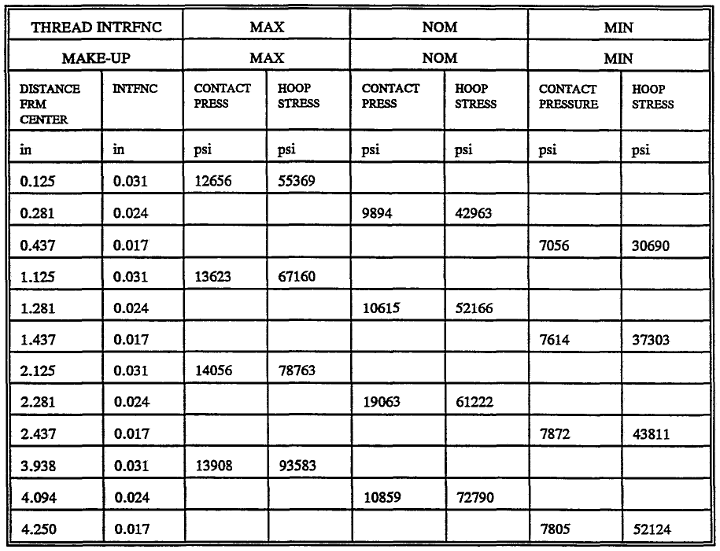
\includegraphics[width=0.3\textwidth]{results/test0.png}} &
\centerline{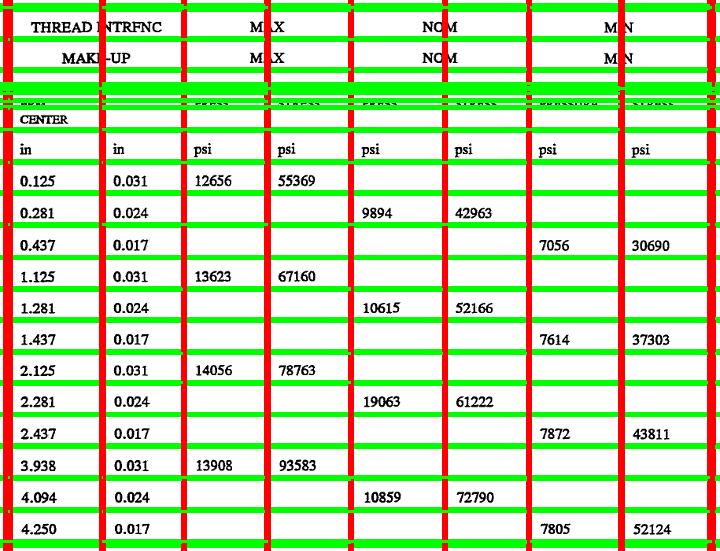
\includegraphics[width=0.3\textwidth]{results/test0-tab.png}} &
\centerline{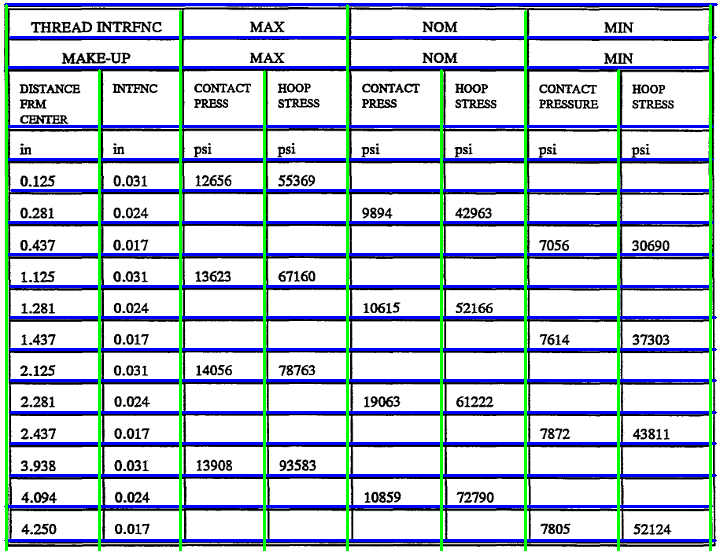
\includegraphics[width=0.3\textwidth]{results/test0-our.png}}\\\hline\hline

\def\arraystretch{1}& \\\def\arraystretch{30}
\centerline{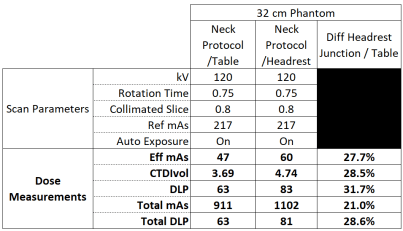
\includegraphics[width=0.3\textwidth]{results/test1.png}} &
\centerline{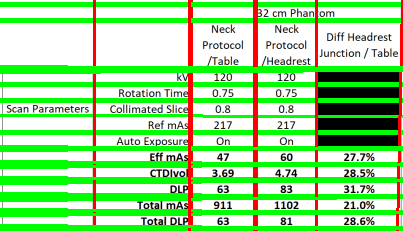
\includegraphics[width=0.3\textwidth]{results/test1-tab.png}} &
\centerline{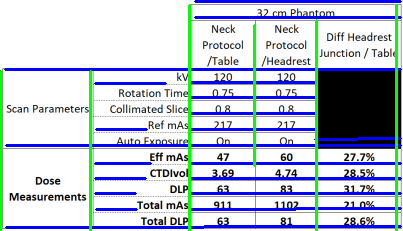
\includegraphics[width=0.3\textwidth]{results/test1-our.png}} \\\hline\hline

\def\arraystretch{1}& \\\def\arraystretch{10}
\centerline{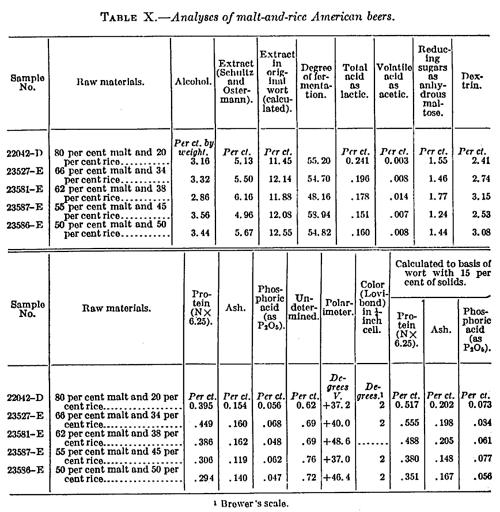
\includegraphics[width=0.3\textwidth]{results/test2.jpg}} &
\centerline{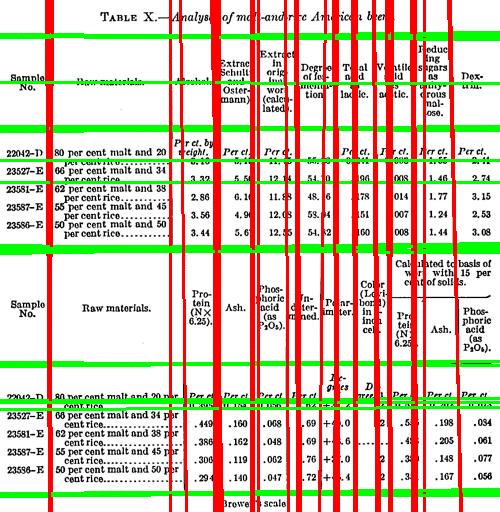
\includegraphics[width=0.3\textwidth]{results/test2-tab.jpg}} &
\centerline{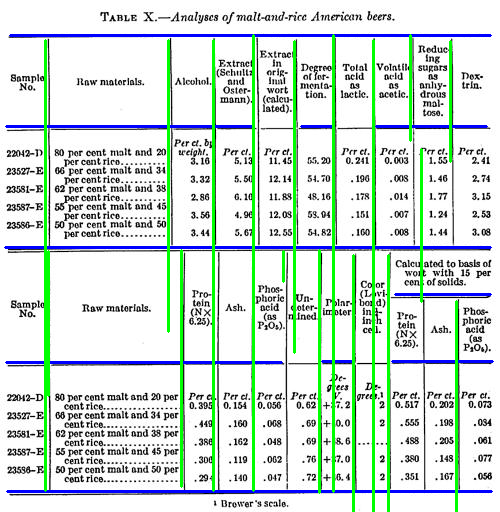
\includegraphics[width=0.3\textwidth]{results/test2-our.png}} \\\hline\hline

\def\arraystretch{1}& \\\def\arraystretch{30}
\centerline{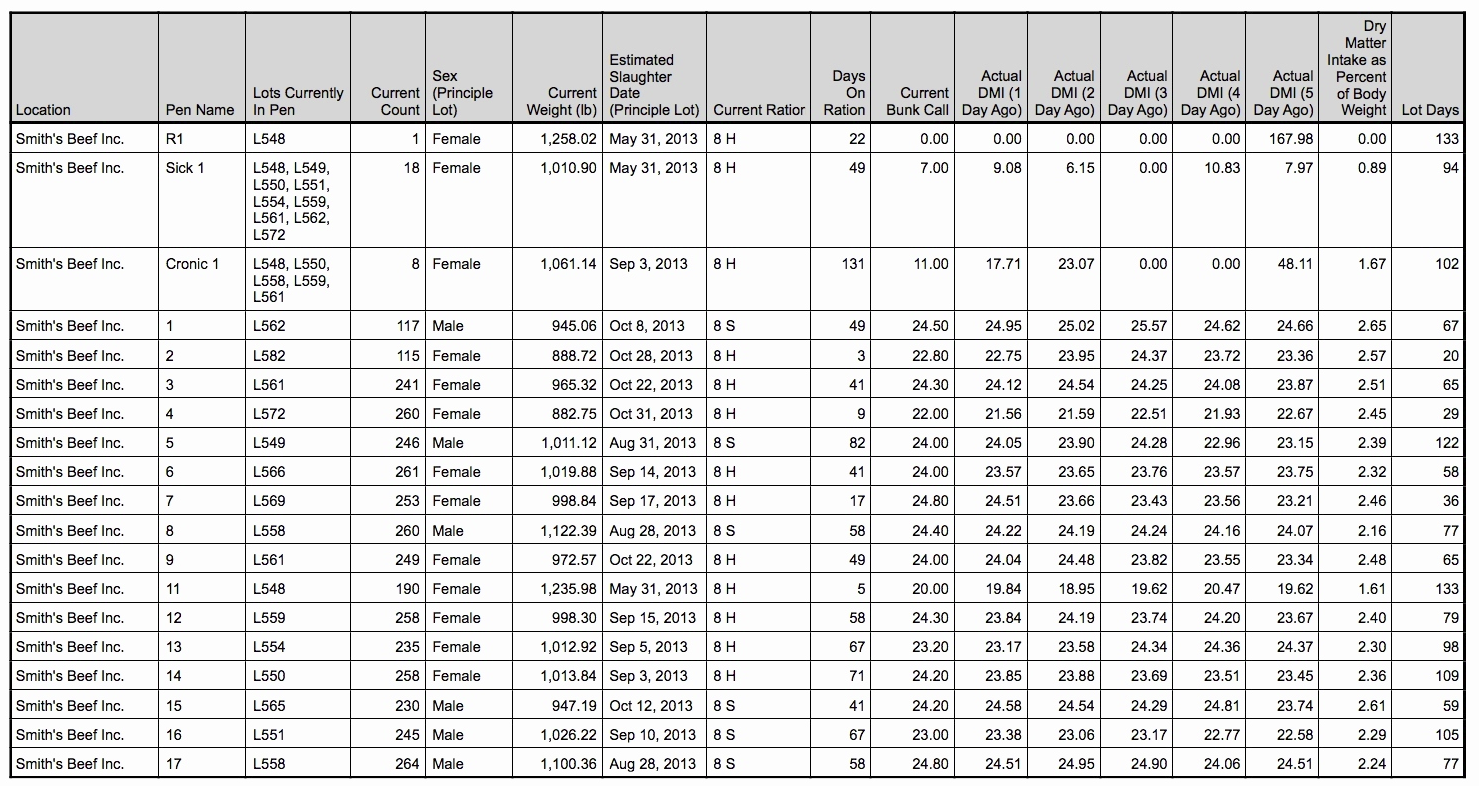
\includegraphics[width=0.3\textwidth]{results/test5.png}} &
\centerline{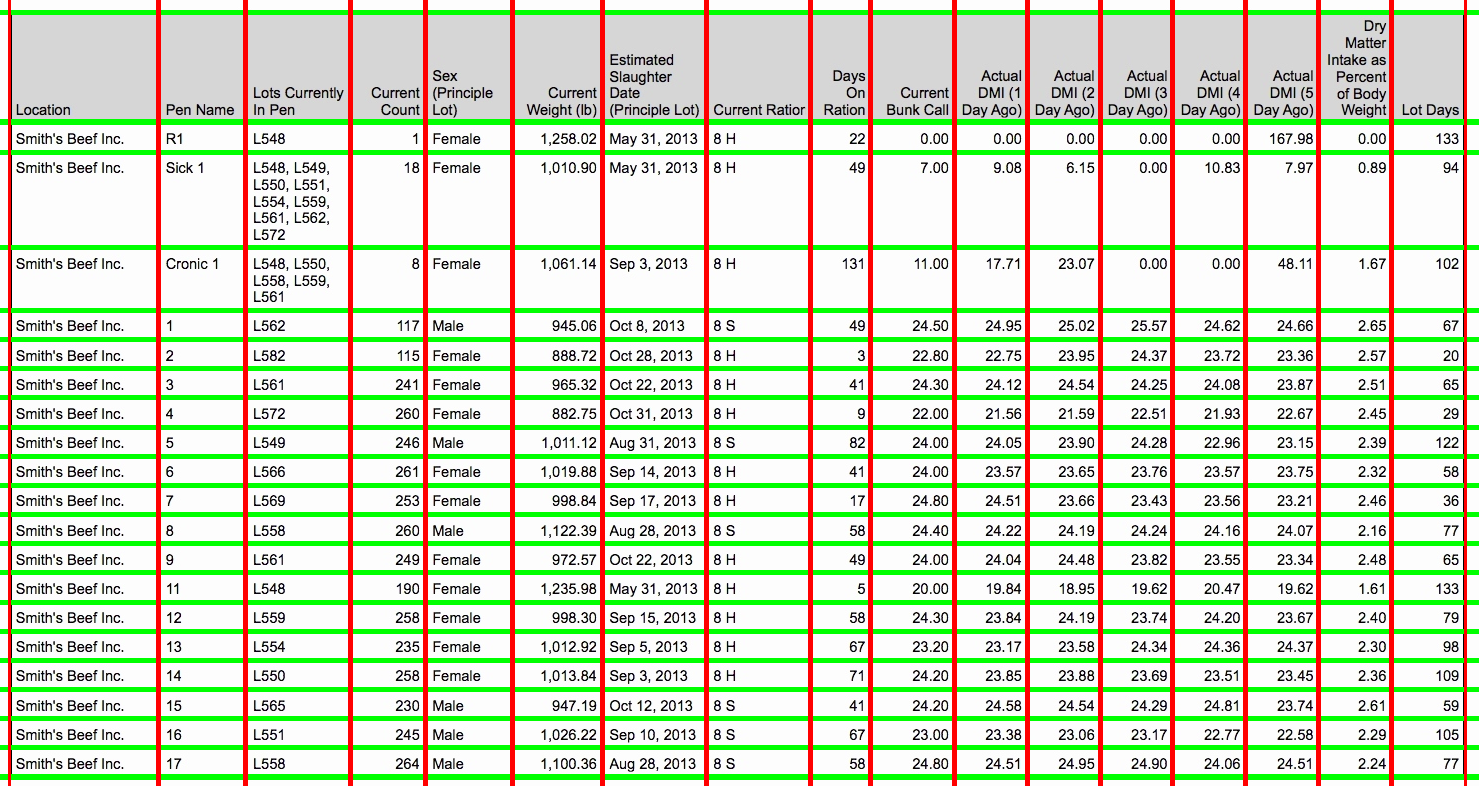
\includegraphics[width=0.3\textwidth]{results/test5-tab.png}} &
\centerline{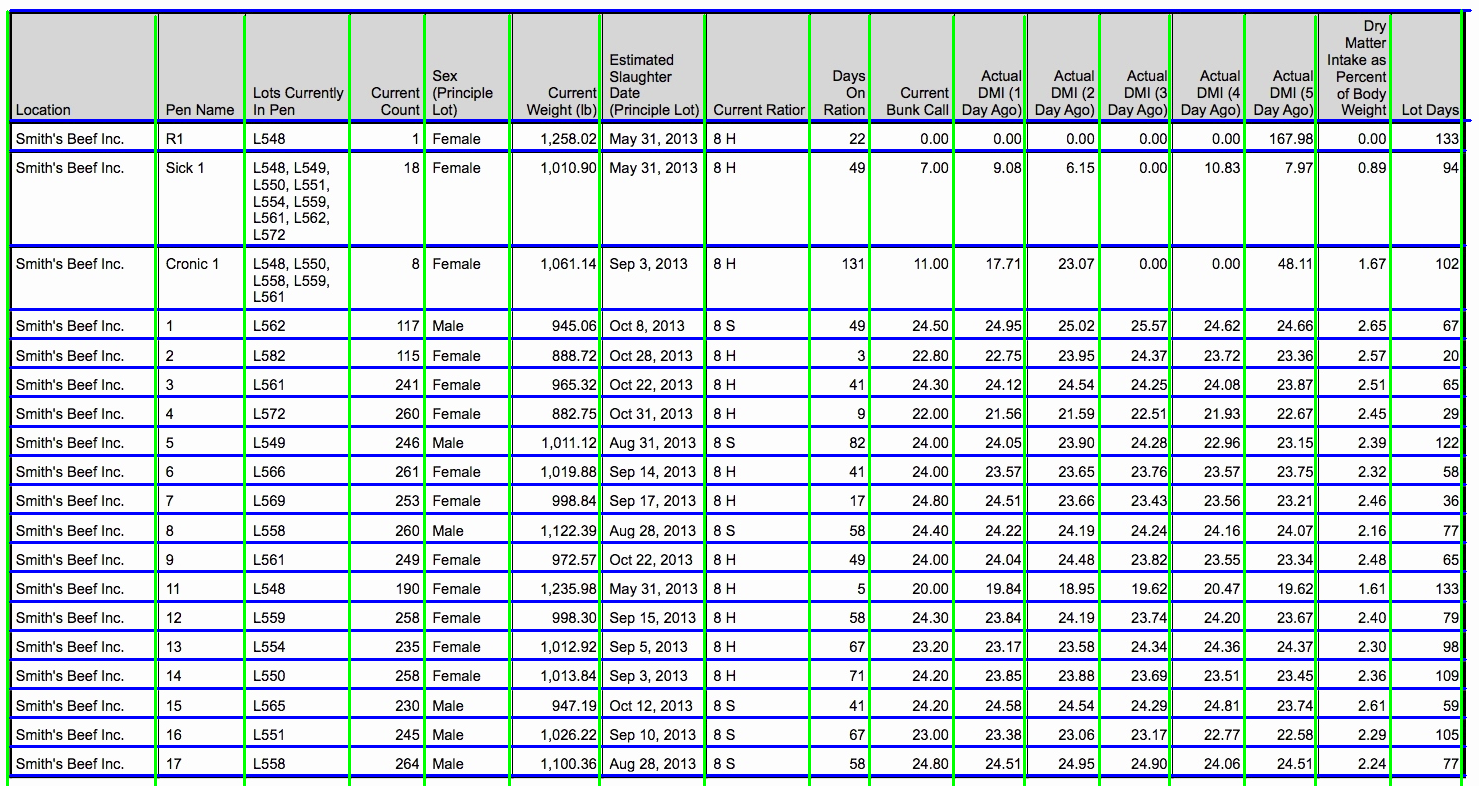
\includegraphics[width=0.3\textwidth]{results/test5-our.png}} \\\hline\hline

\hline
\end{tabular}
\end{table*}

\section*{Conclusion and Future work}
Few of the future extensions of this project are listed below:
\begin{itemize}
    \item Auto image formatting (like output provided by CamScanner\cite{camscanner}, FastScanner\cite{fastscanner}, etc)
    \item De-skewing of slightly rotated image.
    \item Cell boundary confirmation using joints.
    \item Bolding edges through contrast manipulation.
\end{itemize}
% references section

% can use a bibliography generated by BibTeX as a .bbl file
% BibTeX documentation can be easily obtained at:
% http://www.ctan.org/tex-archive/biblio/bibtex/contrib/doc/
% The IEEEtran BibTeX style support page is at:
% http://www.michaelshell.org/tex/ieeetran/bibtex/
%\bibliographystyle{IEEEtran}
% argument is your BibTeX string definitions and bibliography database(s)
%\bibliography{IEEEabrv,../bib/paper}
%
% <OR> manually copy in the resultant .bbl file
% set second argument of \begin to the number of references
% (used to reserve space for the reference number labels box)

\bibliographystyle{IEEEtran}
\bibliography{main}
\section{Appendix}\label{appendix-title-1b8525ae1891}
\subsection{The Name `Tabla'}
After much deliberation and spending more time on naming than actually working on the project we decided to name our project `Tabla', it's derived from the word \inline{table} but has been modified to represent our framework. The letter \inline{e} has been dropped (which signified \textbf{e}ffort that the user had to put in) and has been replaced by \inline{a} to create \inline{tabla}. The letter \inline{a} in the new name signifies the framework's accessibility. This is demonstrated much clearly in the Figure \ref{fig:naming}.


\begin{figure}[!t]
\centering
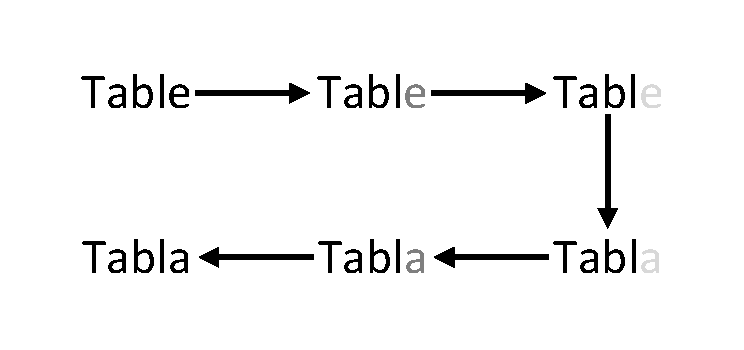
\includegraphics[width=2.5in]{figures/naming.pdf}
\caption{Naming of our framework.}
\label{fig:naming}
\end{figure}
     
\end{document}